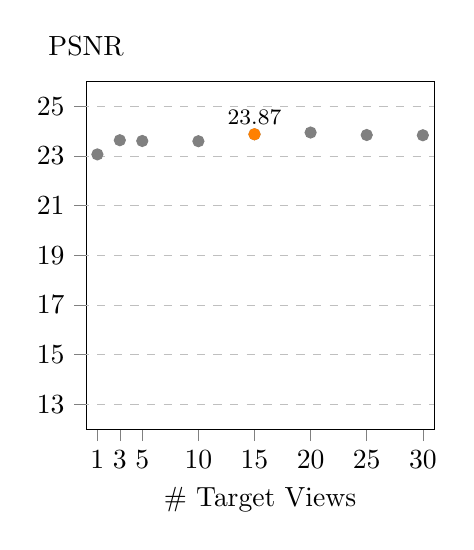
\begin{tikzpicture}

\definecolor{color0}{rgb}{0.12156862745098,0.466666666666667,0.705882352941177}

\begin{axis}[
    every axis y label/.style={at={(current axis.north west)},above=2mm},
    width=6cm, height=6cm,
    legend cell align={left},
    legend style={fill opacity=1.0, draw opacity=1, text opacity=1, draw=none, column sep=2pt, very thick, anchor=south east, at={(0.98,0.02)}, legend columns=2, font=\footnotesize},
    tick align=outside,
    tick pos=left,
    xlabel={\# Target Views},
    xmin=0, xmax=31,
    xtick={1,3,5,10,15,20,25,30},
    ytick={13, 15, 17, 19, 21, 23, 25},
    ylabel={PSNR},
    ymin=12, ymax=26,
]
\addplot[line width=0.2pt, dashed, lightgray] coordinates {(-0.5,11)(31,11)};
\addplot[line width=0.2pt, dashed, lightgray] coordinates {(-0.5,13)(31,13)};
\addplot[line width=0.2pt, dashed, lightgray] coordinates {(-0.5,15)(31,15)};
\addplot[line width=0.2pt, dashed, lightgray] coordinates {(-0.5,17)(31,17)};
\addplot[line width=0.2pt, dashed, lightgray] coordinates {(-0.5,19)(31,19)};
\addplot[line width=0.2pt, dashed, lightgray] coordinates {(-0.5,21)(31,21)};
\addplot[line width=0.2pt, dashed, lightgray] coordinates {(-0.5,23)(31,23)};
\addplot[line width=0.2pt, dashed, lightgray] coordinates {(-0.5,25)(31,25)};



\addplot [draw=gray, fill=gray, mark=*, only marks, mark size=2pt]
table{%
x  y
1 23.06
3 23.63
5 23.60
10 23.59
15 23.87
20 23.94
25 23.84
30 23.83
50 23.89
100 24.04
};

\addplot [draw=orange, fill=orange, mark=*, only marks, mark size=2pt]
table{%
x  y
15 23.87
};
\node[above] at (axis cs:15, 23.87) {\footnotesize 23.87};

\end{axis}

\end{tikzpicture}
